\documentclass[12pt]{article}
\usepackage{amsmath}
\usepackage{gensymb}
\usepackage{float}
\usepackage{graphicx}
\usepackage{graphics}
\graphicspath{{/storage/self/primary/Download/latexnew/fig}}
\graphicspath{{/storage/self/primary/Download/latexnew/table}}
\let\vec\mathbf
\providecommand{\brak}[1]{\ensuremath{\left(#1\right)}}
\begin{document}
\title{\textbf{VECTOR}}
\date{}
\maketitle
\textbf{Question :} Construct a triangle $APB$ in which $BC = 7cm$,$\angle B = 75\degree$ and $AB+AC = 13cm$.

\textbf{Figure :}
\begin{figure}[H]
    \centering
          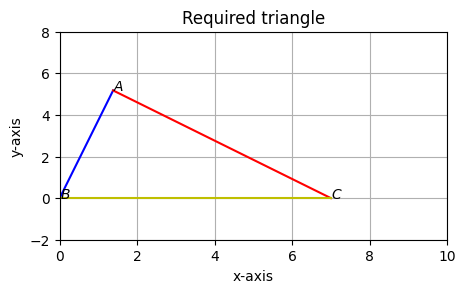
\includegraphics[width=\columnwidth]{fig/2.png}
    \caption{}
    \label{fig:fig:1}
\end{figure}

\textbf{Solution :}
\begin{table}[H]
    \centering
       \begin{tabular}{|c|c|c|}
    \hline
    \textbf{Input Parameters} &\textbf{Description} &\textbf{Value} \\
    \hline
     $\vec{O}$& Center(at origin)&$\vec{0}$\\
     \hline
 $r$ & Radius &1\\
 \hline
 $\theta$&-&$100\degree$\\
 \hline
 $\alpha$&-&$165.4\degree$\\
 \hline
 $\beta$&-&$5\degree$\\
 \hline
  \end{tabular}

    \caption{Table of input parameters}
    \label{tab:tab:1}
\end{table} 
\begin{table}[H]
    \centering
    \begin{tabular}{|c|c|c|}
    \hline
        \textbf{Output Parameters} &\textbf{Description} &\textbf{Value} \\
\hline
          $\vec{Q}$ & Point &$\myvec{\cos{\theta_1}\\\sin{\theta_1}}$\\
          \hline
          $\vec{P}$ & Point &$\myvec{\cos{\theta_2}\\\sin{\theta_2}}$ \\
         \hline
          $\vec{R}$ & Point &$\myvec{\cos{\theta_3}\\sin{\theta_3}}$ \\
         \hline
    \end{tabular}


  \caption{Table of output parameters}
    \label{tab:tab:2}
\end{table}
From cosine rule,
\begin{align}
  b^2&=a^2+c^2-2ac\cos{\angle B} \\
  or,b^2&=a^2+c^2-2ac\brak{\frac{\sqrt{3}-1}{2\sqrt{2}}}\\
  or,b^2-c^2 &=a^2-ac\brak{\frac{\sqrt{3}-1}{\sqrt{2}}}\\
  or,\brak{b+c}\brak{b-c}&=a^2-ac\brak{\frac{\sqrt{3}-{1}}{\sqrt{2}}}\\
  or,13\brak{b-c}&=49-7c\brak{\frac{\sqrt{3}-{1}}{\sqrt{2}}}\\
  or,13b+\brak{-13+7\brak{\frac{\sqrt{3}-1}{\sqrt{2}}}}c&=49\\
  b+c&=13\end{align}
From \brak{6},\brak{7} \\
\begin{align}
&\left[
\begin{array}{cc|c}
13&-13+7\brak{\frac{\sqrt{3}-1}{\sqrt{2}}}&49\\
1&1&13\end{array}
\right]\\
\xrightarrow{R_1'=R_1/13}&\left[
\begin{array}{cc|c}
1&\frac{-13+7\brak{\frac{\sqrt{3}-1}{\sqrt{2}}}}{13}&\frac{49}{13}\\
1&1&13\end{array}
\right]\\
 \xrightarrow{R_2'= R_2-R_1}&\left[
\begin{array}{cc|c}
1&\frac{-26+7\sqrt{6}-7\sqrt{2}}{26}&\frac{49}{13}\\
0&\frac{52-7\sqrt{6}+7\sqrt{2}}{26}&\frac{120}{13}\end{array}
\right]\\
  \xrightarrow[R_2"=R_2'\brak{\frac{26}{52-7\sqrt{6}+7\sqrt{2}}}]{R_1"= R_1'-R_2'\brak{\frac{-26+7\sqrt{6}-7\sqrt{2}}{52-7\sqrt{6}+7\sqrt{2}}}}&\left[
\begin{array}{cc|c}
1&0&\frac{436-91\sqrt{6}+91\sqrt{2}}{52-7\sqrt{6}+7\sqrt{2}}\\
0&1&\frac{240}{52-7\sqrt{6}+7\sqrt{2}}\end{array}
\right]\\
 \begin{bmatrix}
     b\\c
 \end{bmatrix}&=\begin{bmatrix}
   \frac{436-91\sqrt{6}+91\sqrt{2}}{52-7\sqrt{6}+7\sqrt{2}}\\\frac{240}{52-7\sqrt{6}+7\sqrt{2}}
 \end{bmatrix}
\end{align}
Therefore,
\begin{align}
    \Vec{A}&=c\begin{bmatrix}
        \cos{\theta}\\\sin{\theta}
    \end{bmatrix}\\
    &=\frac{240}{52-7\sqrt{6}+7\sqrt{2}}\begin{bmatrix}
        \cos{75\degree}\\\sin{75\degree}
    \end{bmatrix}\\
    &=\begin{bmatrix}
        1.388\\5.18
    \end{bmatrix}\\
\end{align}

\end{document}
